\documentclass{coursework}

\title{勘探地球物理新进展\\课程作业}%名称(这门课作业有点多)
\studentName{你的名字}               %姓名
\studentID{你的学号}              %学号
\teacherName{任课教师}               %任课教师
				  
\major{17级地球物理班}             %专业班级

%%%每个章节分别列出各自的参考文献,采用multibib宏包,具体用法需要百度或goole一下
%\usepackage{multibib}
%\newcites{one}{参考文献(作业一)}


%%%windows系统下如果想用Times New Roman字体,可以uncomment下面三句,Linux下不适用
%\setmainfont{Times New Roman}
%\setmonofont{Courier New}
%\setsansfont{Arial}

\begin{document}
	\maketitle	
	\section{作业一}
	鲁迅说过:“这个世界不只有眼前的苟且,还有明天的苟且,后天的苟且,以及陈老师的4w字作业”\citep{luxun}。
	\subsection{论述航空电磁法仪器进展}
	\citep{Fountain1998,AUKEN201747}。
	
	
	插入一个公式
	\begin{equation}\label{equ:Fma}
	\mathbf{F}=m\frac{d^2\mathbf{r}}{dt^2}
	\end{equation}
	引用公式\eqref{equ:Fma}
	
	插入一个图
	\begin{figure}[H]
		\centering
		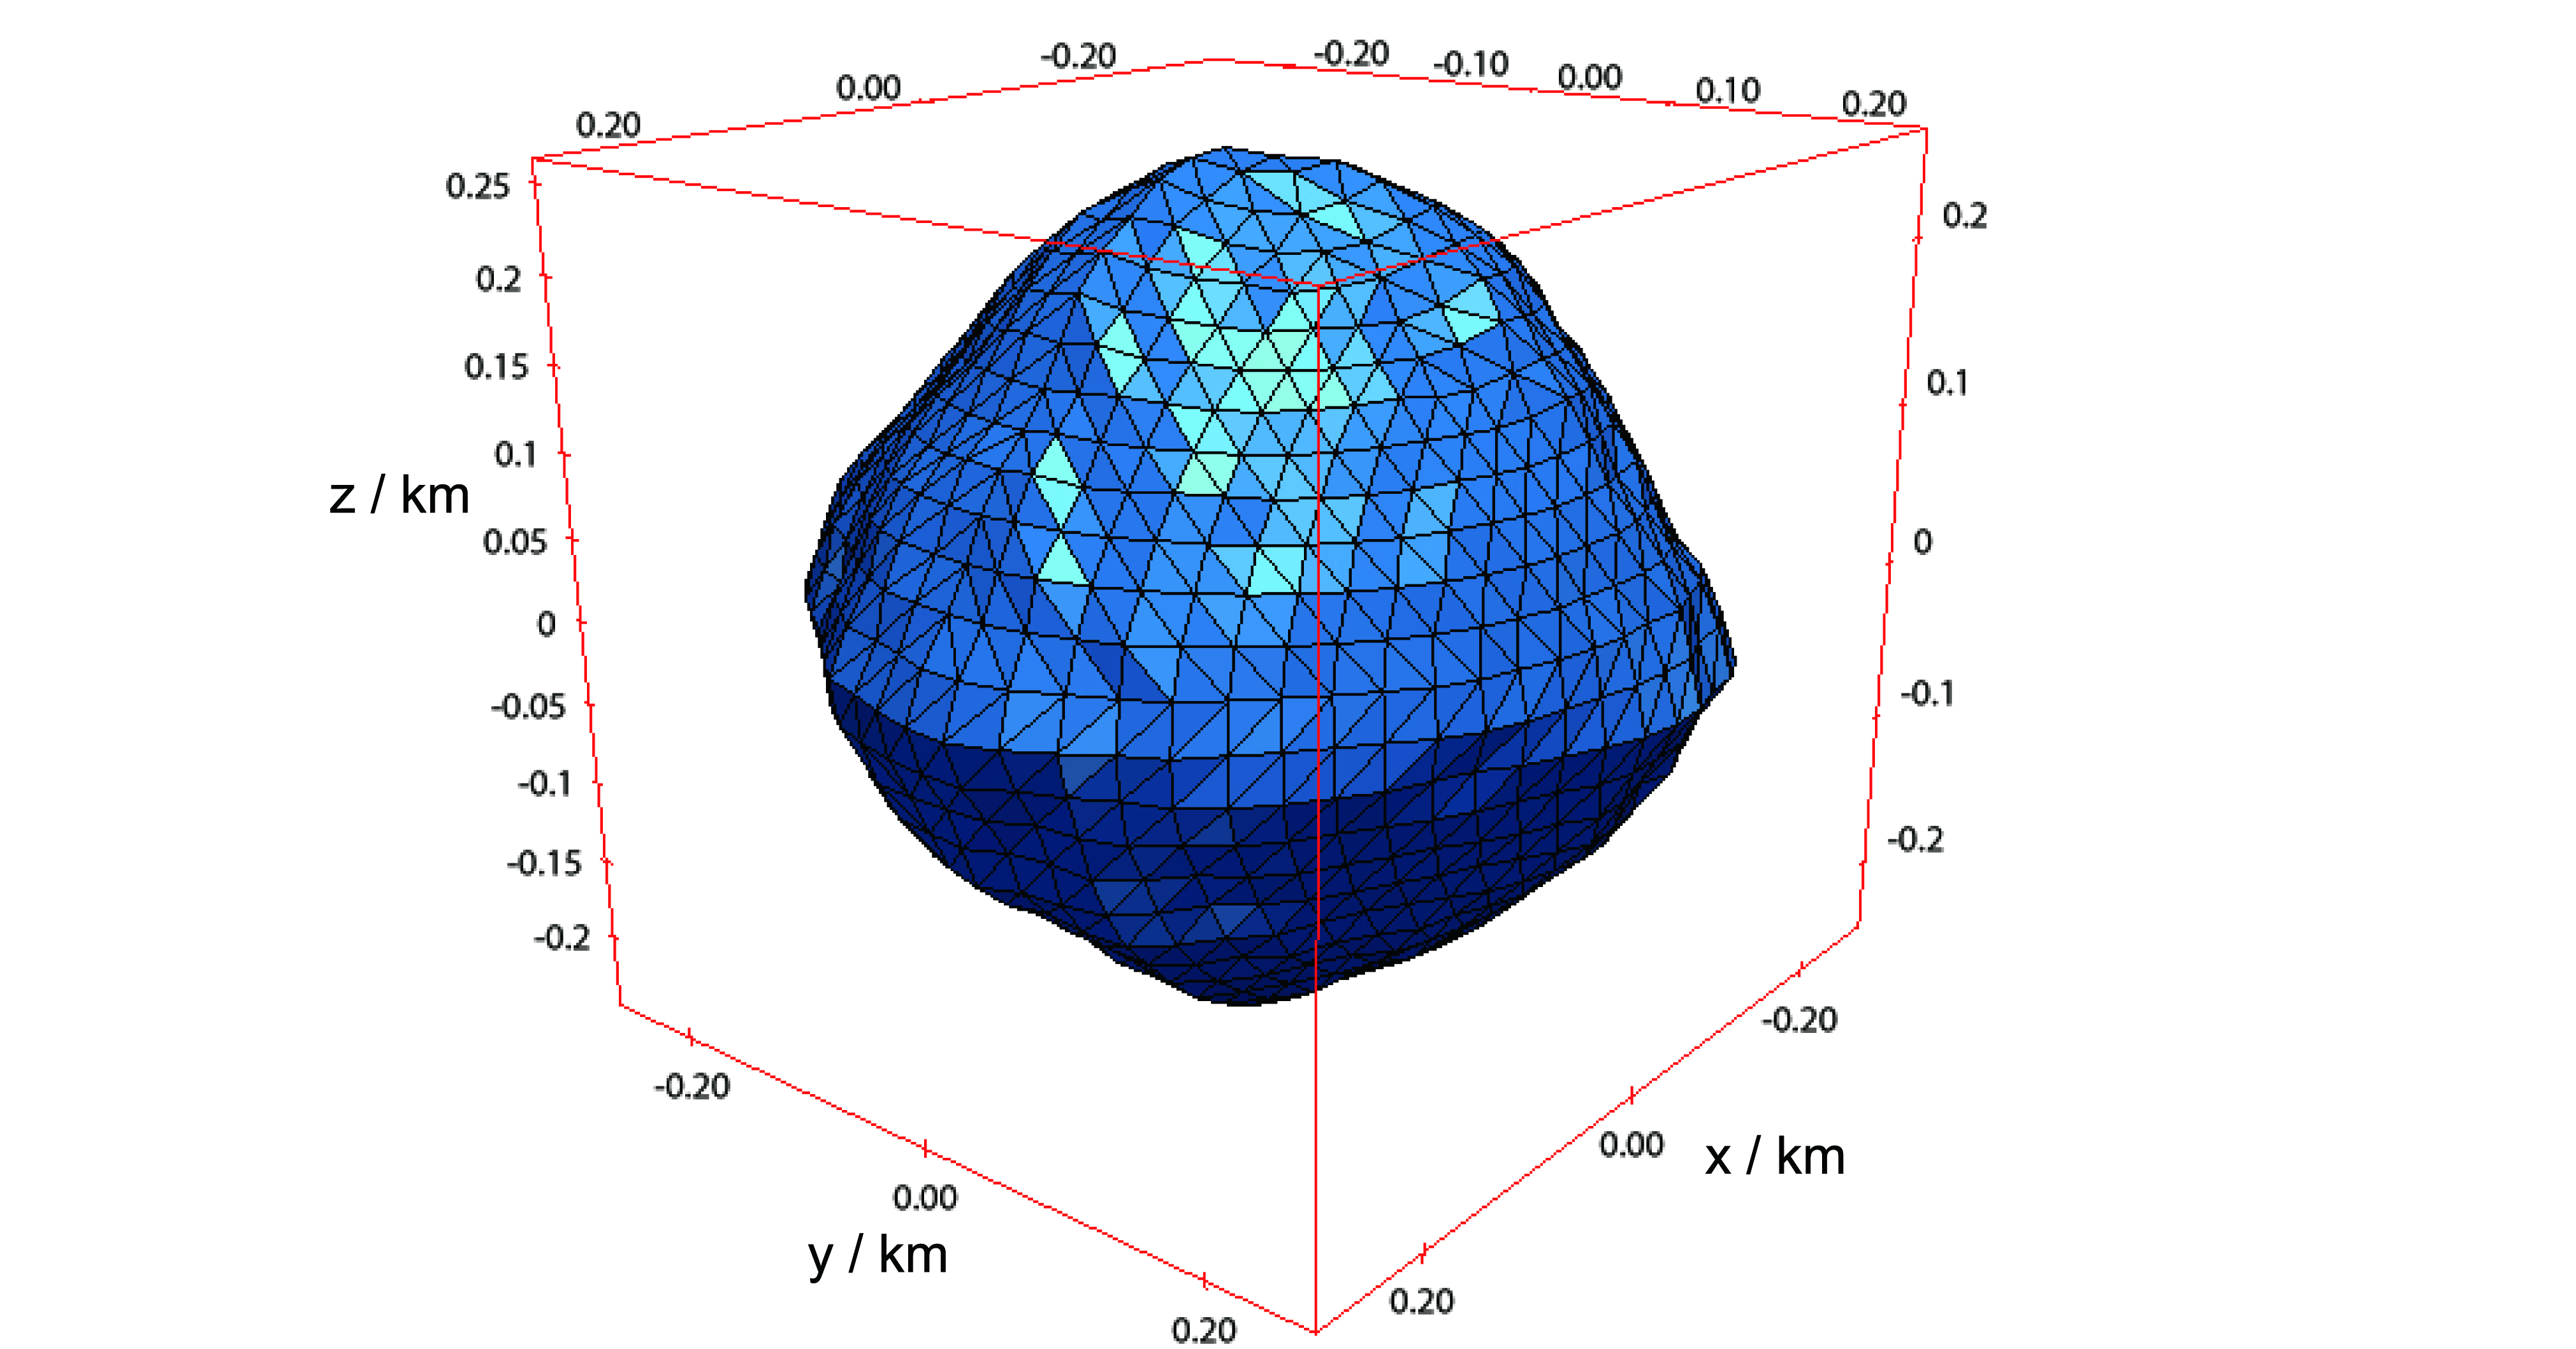
\includegraphics[width=0.8\linewidth]{fig/1.jpg}
		\caption{图名字,黑体5号}\label{fig:1}
	\end{figure}
	引用图(\ref{fig:1})

	插入表
	\begin{table}[H]
		\centering
		\caption{表名字,黑体5号}\label{tab:1}
		\begin{tabular}{cc}
			\toprule
			x (m)&y (m)  \\ 
			\midrule 
			1.000&2.000  \\ 
			\hline 
			3.000&4.000  \\ 
			\bottomrule
		\end{tabular} 
	\end{table}
	引用表(\ref{tab:1})	
	
	......
	\subsection{论述地面电磁法仪器进展}
	......
	\subsection{论述大规模高密度电磁探测的意义和作用}
	......
	\subsection{论述频谱激电进展及发展趋势}
	......
	
	\section{作业二}
	\subsection{论述三维MT/AMT在地热勘探中的应用}
	......	
	\subsection{论述三维MT/AMT在活火山研究中的应用}
	......	
	\subsection{论述决定岩矿石频谱激电响应的因素}
	......	
	\subsection{论述频谱激电区分矿与非矿原理}
	......	

	\section{作业三}
	\subsection{论述影响TEM浅层勘探效果的因素}
	......
	\subsection{论述IP效应对TEM观测的影响}
	......	
	\subsection{如何提高浅层瞬步电磁仪的性能?}
	......
	\subsection{如何识别和利用IP和SPM效应?}
	......
	\section{作业四}
	\subsection{论述航空瞬变电磁(ATEM)响应中IP效应研究进展}
	......
	\subsection{论述三维TEM正反演进展}
	......
	\subsection{论述正则化反演的地质地球物理意义}
	......
	\subsection{论述在已知矿体形态矿床开展多方法地球物理勘探试验的意义}
	......
	\section{作业五}
	\subsection{论述电阻率法和电磁法联合反演进展}
	......
	\subsection{论述电阻率法和电磁法联合反演的物理基础}
	......
	\subsection{论述地震、电阻率法、电磁法和地震雷达联合反演的物理基础}
	......
	\subsection{论述多方法联合反演的原理与进展}
	......
	\section{作业六}
	\subsection{论述电法和电磁法勘探(包括航空、地面、井地和井间电法电磁法)在油气勘探中的应用}
	......
	\subsection{论述海洋电磁法在油气勘探中的应用}
	......
	\subsection{论述地震与电磁法联合勘探进展}
	......
	\subsection{论述地震与电磁法联合勘探进展}
	......
	\section{作业七}
	\subsection{论述磁法反演新进展}
	......
	\subsection{论述重力反演新进展}
	......
	\subsection{论述三维地震数据断层自动解释新进展}
	......
	\subsection{论述三维地震波阻抗反演进展}
	......
	\section{作业八}
	\subsection{论述三维地震数据地质构造自动解释新进展}
	......
	\subsection{论述三维地震与测井数据联合解释新进展}
	......
	\subsection{论述大规模并行计算在地球物理数据处理、反演与解释中的应用}
	......
	\subsection{论述大规模地球物理并行正反演基本原理(包括问题分解与综合方法、并行化方法、并行效率分析等)}
	......
	\subsection{论述激电效应的机理}
	......
	
	
	\bibliographystyle{model5-names.bst}%参考文献格式,model5-names.bst是爱思唯尔的提供的参考文献格式之一,这里也可以换成其他的
	\bibliography{mybibfile}%把需要用到的参考文献写在mybibfile.bib文件中
\end{document}
